% Springer LNCS / AIST 2026 camera-ready version
\documentclass[runningheads,a4paper]{llncs}

\usepackage{cmap}
\usepackage[utf8]{inputenc}
\usepackage[T1]{fontenc}
\usepackage[english]{babel}
\usepackage{graphicx}
\usepackage{booktabs}
\usepackage{tabularx}
\usepackage{array}
\usepackage{amsmath}
\usepackage{amssymb}
\usepackage{url}
\usepackage{placeins}
\usepackage{float}
\usepackage{microtype}

\newcommand{\schwartz}{Schwartz-10}
\newcommand{\val}[1]{\textsc{#1}}
\newcommand{\acc}{Acc@1}
\newcommand{\accthree}{Acc@3}
\newcommand{\dataset}{Russian Schwartz-10 recognition set}

\begin{document}
\raggedbottom

\title{Which Values Do LLMs Confuse? A Schwartz-Based Recognition Study}
\titlerunning{Which Values Do LLMs Confuse?}
\author{Andrei Chetvergov\inst{1,2}\thanks{Corresponding author.} \and
Stepan Ukolov\inst{1,2} \and
Timofei Sivoraksha\inst{1,2} \and
Alexander Evseev\inst{1,2} \and
Mikhail Solovev\inst{1,2} \and
Valeriia Kuschenko\inst{2} \and
Maria Chistyakova\inst{2} \and
Sergey Bolovtsov\inst{1,2}}
\authorrunning{A. Chetvergov et al.}
\institute{Ivannikov Institute for System Programming of the Russian Academy
of Sciences, Moscow, Russia \and
Russian Presidential Academy of National Economy and Public Administration,
Moscow, Russia\\
\email{chetvergov-as@ranepa.ru}}
\maketitle

\begin{abstract}
Large language models are increasingly evaluated through the values they endorse, but such evaluations presuppose that models can identify the value expressed in a concrete situation. We study this prerequisite as controlled top-1 recognition over Schwartz's ten basic values. Our evaluation set contains 1,000 Russian situational texts, balanced across the ten values and independently labeled by two human annotators per item. We evaluate 21 instruction-tuned LLM runs under a fixed ranked-response protocol; 20 runs with reliable outputs form the semantic panel. Pooled \acc{} is 0.683 and \accthree{} is 0.892, showing that models often locate the correct motivational region while ranking close alternatives unstably. Adjacent values account for 50.9\% of semantic errors, compared with 24.4\% under a checkpoint-specific null. Eight directed confusions recur across checkpoints and human-confirmed subsets. Several are strongly asymmetric---including \val{Universalism}$\rightarrow$\val{Benevolence}, \val{Tradition}$\rightarrow$\val{Conformity}, and \val{Security}$\rightarrow$\val{Power}---whereas \val{Stimulation}--\val{Hedonism} forms a bidirectional boundary. Their severity is checkpoint-specific and can bias higher-order value profiles. The results motivate value-recognition evaluation that combines exact accuracy, ranked recovery, and directed error analysis.
\keywords{large language models \and human values \and Schwartz values \and
value recognition \and Russian NLP \and model evaluation \and human validation}
\end{abstract}

\section{Introduction}

Human values are increasingly used to evaluate large language models (LLMs): systems are compared by value orientations, moral choices, pluralistic judgments, and value-informed behavior. These evaluations depend on a simpler capability that is rarely isolated. Before asking whether a model endorses or follows a value, one should establish whether it can recognize which value is expressed in ordinary language.

Recognition errors matter because predicted value labels can become features for profiling, routing, recommendation, policy analysis, or personalized intervention. A systematic \val{Universalism}$\rightarrow$\val{Benevolence} shift can reduce a demand for equal access to a story of charitable care; \val{Conformity}$\rightarrow$\val{Security} can turn normative compliance into threat avoidance; and \val{Security}$\rightarrow$\val{Power} can read protective action as domination. These examples make the direction of an error more informative than a generic accuracy loss.

\paragraph{Schwartz-10 in brief.}
Schwartz's circumplex arranges ten values so that neighboring positions express compatible motives and opposite positions express competing priorities~\cite{schwartz1992universals,schwartz2012refining}. Openness to Change comprises \val{Self-Direction} (independent thought and action), \val{Stimulation} (novelty and excitement), and \val{Hedonism} (pleasure); Self-Enhancement comprises \val{Achievement} (success through competence) and \val{Power} (status and control); Conservation comprises \val{Security} (safety and stability), \val{Conformity} (restraint under social norms), and \val{Tradition} (respect for inherited customs); Self-Transcendence comprises \val{Benevolence} (welfare of close others) and \val{Universalism} (welfare of all people and nature). Recognition therefore requires both locating the broad motivational region and distinguishing nearby motives. A single accuracy score can conceal the more diagnostic question posed by our title: \emph{which values does a model confuse, in which direction, and more often than expected from its general label preferences?}

We study primary-value recognition in short Russian situational texts. Each model returns a ranked prediction over \schwartz{}. Russian provides the empirical setting; the object of analysis is the structure of value recognition and confusion. Figure~\ref{fig:overview} summarizes the task.

The study addresses three research questions:
\begin{itemize}
    \item \textbf{RQ1 -- Recognition and ranked recovery.} How accurately do instruction-tuned LLMs recognize primary Schwartz values, which values are hardest, and how often does the reference remain at ranks 2--3 after a top-1 disagreement?
    \item \textbf{RQ2 -- Directed confusion and checkpoint heterogeneity.} Which directed boundaries exceed checkpoint-specific label-preference baselines, reproduce across checkpoints and family exclusions, and form distinct model-specific error fingerprints?
    \item \textbf{RQ3 -- Human robustness and profile distortion.} Do the conclusions persist on independently confirmed items, what semantic mechanisms recur, and how do fine-grained errors alter higher-order motivational profiles?
\end{itemize}

Our contributions are fourfold. First, we formulate primary-value recognition as a controlled diagnostic task and release a balanced set of 1,000 unique Russian texts with two independent human labels for every item. Second, we separate output reliability, exact recognition, and ranked recovery, and introduce checkpoint-specific fixed-margin inference with replication and leave-one-family-out tests. Third, we characterize eight reproducible directed transitions, expose checkpoint-specific confusion fingerprints, and audit all 62 high-consensus cases for recurring semantic mechanisms. Fourth, we repeat the central analyses on two human-confirmed subsets and quantify the resulting distortion of higher-order value profiles over 20,000 model--text observations.

\begin{figure}[H]
\centering
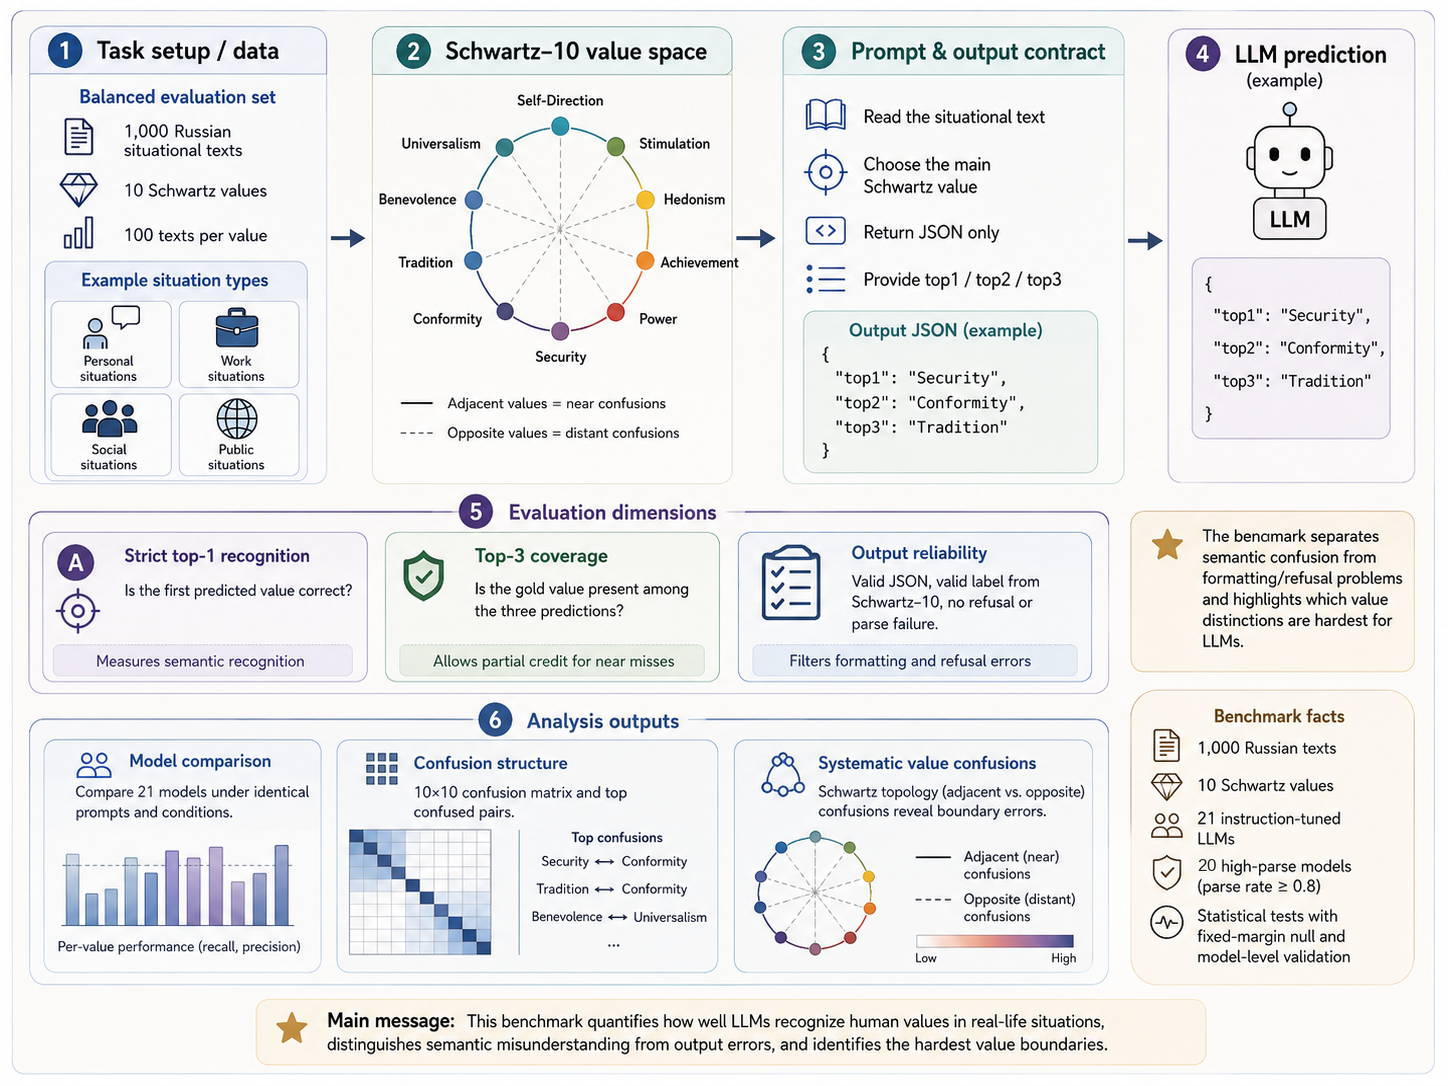
\includegraphics[width=0.96\textwidth]{figures/task_overview.png}
\caption{Task overview. A model maps a situational text to one primary Schwartz value and two alternatives under a fixed ranked-response schema. Evaluation separates output reliability, top-1 recognition, top-3 coverage, and confusion structure.}
\label{fig:overview}
\end{figure}

\section{Related Work}

\paragraph{Value Recognition in Text.}
Webis-ArgValues-22 established value inference from natural-language arguments as an NLP task~\cite{kiesel2022identifying}; ValueEval and the Touche23-ValueEval extension enabled system and per-category comparison over larger multilabel argument collections~\cite{kiesel2023semeval,mirzakhmedova2024touche}. These resources establish values as operational textual categories. Our study adds a compact psychological geometry in which directed boundaries and circumplex distance are directly interpretable.

\paragraph{LLM Value and Scenario Benchmarks.}
ValueBench evaluates orientations and value understanding across many psychometric dimensions~\cite{ren2024valuebench}; Value Kaleidoscope / ValuePrism emphasizes pluralistic rights and duties in situations~\cite{sorensen2024value}; Generative Psychometrics and ValueLlama support scalable value measurement from free text~\cite{ye2025measuring}. INVP studies value priorities in social decisions~\cite{liu2025invp}, ValueActionLens examines the value--action gap~\cite{shen2025valueaction}, and Value Portrait links realistic interactions to human value scores~\cite{han2025portrait}. We isolate a prerequisite shared by these settings: distinguishing the expressed value before interpreting a profile or action.

\paragraph{Annotation Uncertainty and Russian Sources.}
Value expression in natural text is difficult to annotate consistently. Epstein et al. report substantial human and model variation in social-media value ratings~\cite{epstein2025measuring}; Milkova and Rudnev emphasize calibrated non-English Schwartz annotation, expert verification, and error-structure analysis~\cite{milkova2026measuring}. We therefore combine exact agreement between two construction models with complete two-annotator human validation. The candidate pool draws on Russian sensitive-topic and appropriateness data~\cite{babakov2021inappropriate} and TAPE ethics examples~\cite{taktasheva2022tape}; source labels select candidates only. Scenario resources such as ETHICS, Social Chemistry 101, and Moral Stories motivate the use of concrete social situations~\cite{hendrycks2021ethics,forbes2020social,emelin2021moral}.

\section{Task and Dataset}

\subsection{Recognition Task and Response Schema}

For a text $x$, the model returns an ordered top-three tuple
$(\hat y_1,\hat y_2,\hat y_3)$ drawn from the ten Schwartz values; we do not
collect a complete ranking of all ten labels. The primary task is
$x\mapsto\hat y_1$. Models identify the value most salient in the described
situation, independently of their own preferences or any judgment of whether
the situation is morally acceptable. Label names are presented without
definitions or demonstrations. Empty responses, refusals, and responses
without an admissible top-1 label are output failures; semantic metrics use
the extracted top-three tuple, while rationales support the qualitative audit.

\begin{figure}[t]
\centering
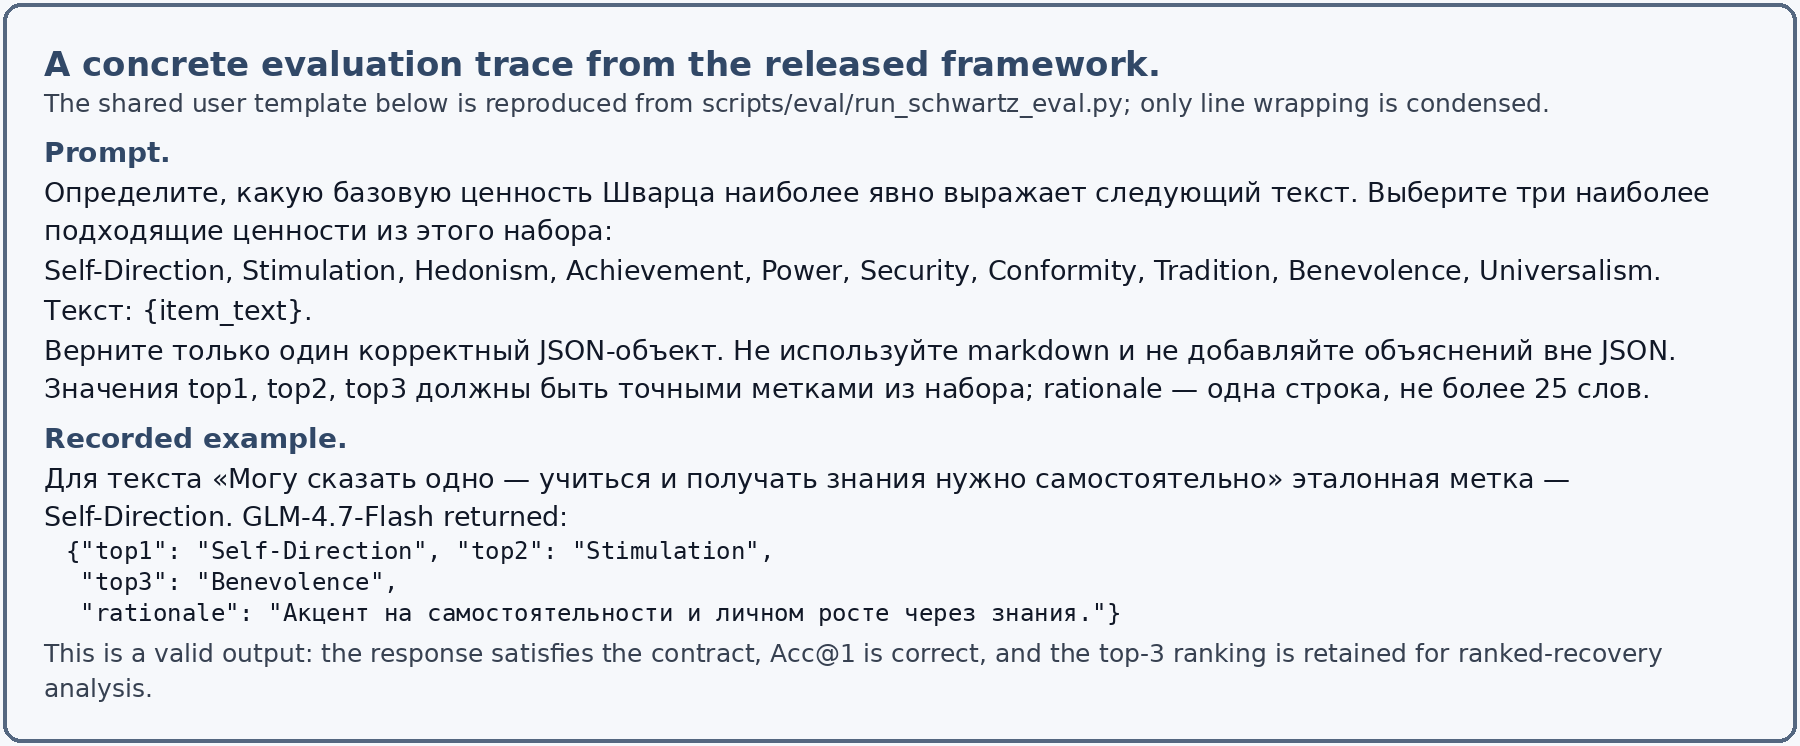
\includegraphics[width=0.96\textwidth]{figures/evaluation_trace.png}
\caption{Evaluation prompt and ranked-response schema. Models return three
distinct labels in rank order plus a short rationale; the parser extracts only
the ordered top-three tuple for semantic metrics.}
\label{fig:prompt}
\end{figure}

\subsection{Candidate Pool and Construction Labels}

The candidate pool contains 70,649 Russian texts from four source slices: 33,303 sensitive-topic texts, 28,931 high-confidence inappropriate messages, a 5,000-item high-confidence appropriate sample, and 3,415 TAPE ethics examples. Source categories are used solely for candidate selection; all final labels belong to the Schwartz-10 space.

The construction stage is shown in Figure~\ref{fig:pipeline}. A specialized ValueLlama annotator labels the candidates; 43,165 items are cross-annotated by GPT-4.1-mini with an explicit \texttt{none} option. Exact top-1 agreement yields 14,516 eligible candidates. For each value, the 100 highest-scoring agreed items are selected subject to a maximum of 60 items from any one source slice. The final set contains 1,000 unique text surfaces, exactly 100 per value: 521 sensitive-topic, 306 high-confidence inappropriate, 85 high-confidence appropriate, and 88 TAPE ethics texts.

\begin{figure}[H]
\centering
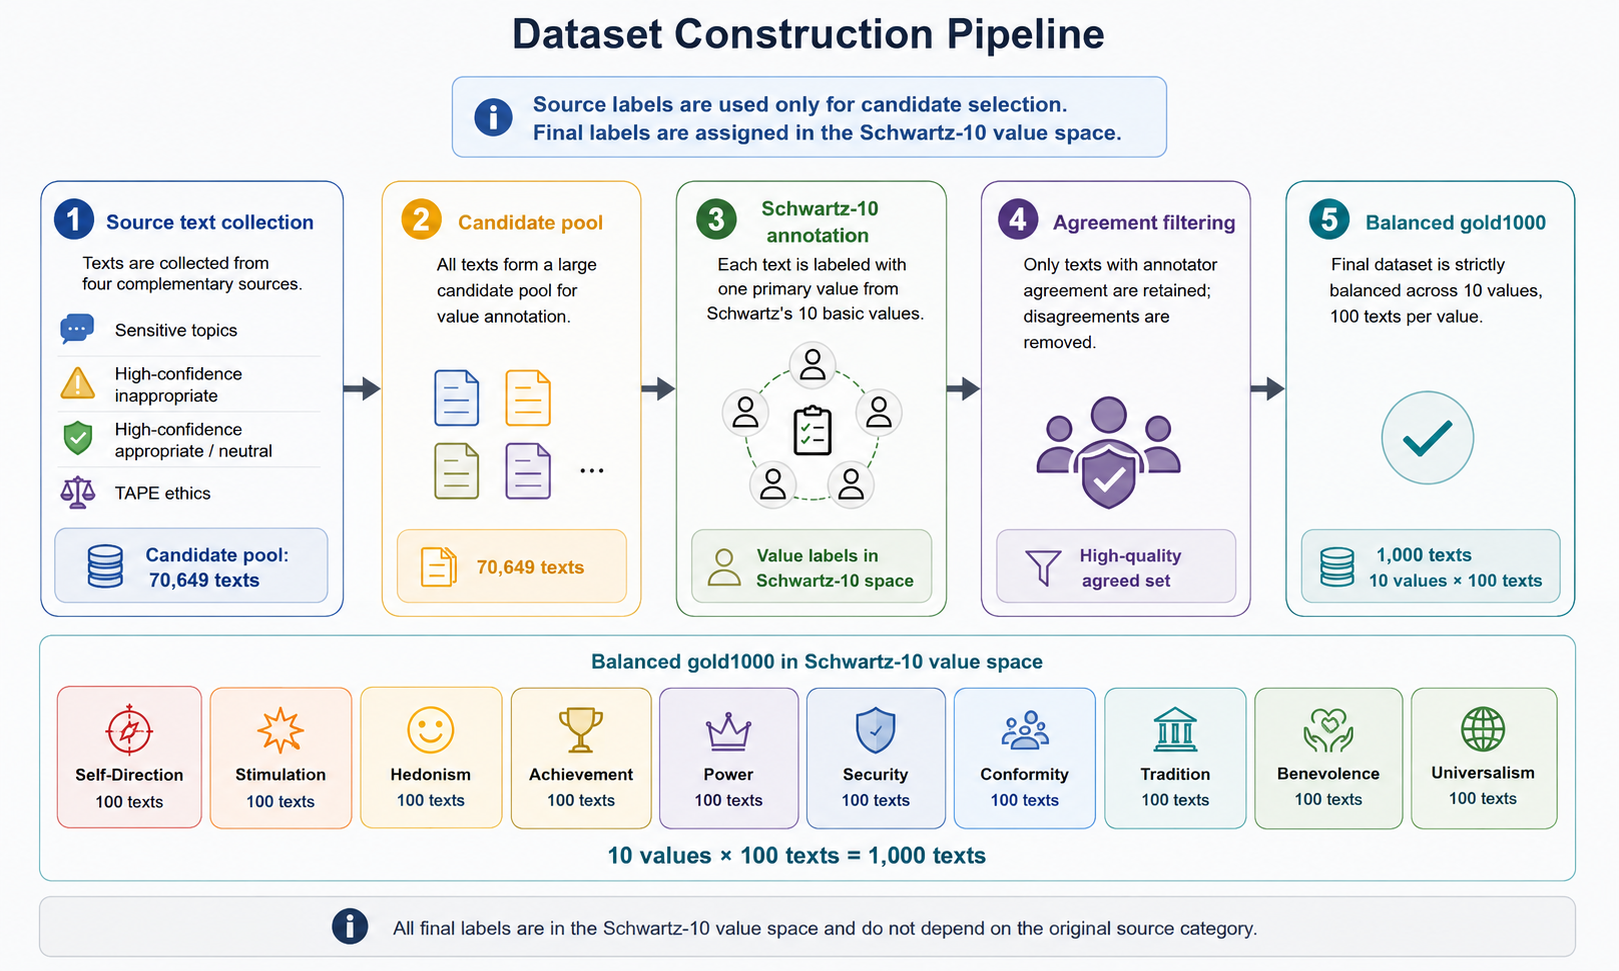
\includegraphics[width=0.98\textwidth]{figures/dataset_pipeline.png}
\caption{Dataset construction. Original source categories select candidates only. Reference labels are assigned in the Schwartz-10 space by two separate construction models and retained under exact top-1 agreement. Every selected item is then independently labeled by two humans.}
\label{fig:pipeline}
\end{figure}

\begin{table}[H]
\caption{Construction-stage selectivity by ValueLlama label. ``Agree'' is exact top-1 agreement with GPT-4.1-mini; \texttt{none} is the GPT abstention rate. The final set then selects 100 items per value.}
\label{tab:constructionaudit}
\centering
\scriptsize
\setlength{\tabcolsep}{4.0pt}
\renewcommand{\arraystretch}{0.94}
\begin{tabular}{@{}lrrrr@{}}
\toprule
Value & Cross-annotated & Agree rate & GPT \texttt{none} & Eligible \\
\midrule
Self-Direction & 3,045 & .200 & .173 & 609 \\
Stimulation & 4,463 & .192 & .312 & 855 \\
Hedonism & 8,487 & .324 & .237 & 2,749 \\
Achievement & 3,748 & .356 & .177 & 1,333 \\
Power & 1,624 & .576 & .132 & 936 \\
Security & 10,288 & .402 & .124 & 4,136 \\
Conformity & 3,622 & .271 & .246 & 981 \\
Tradition & 3,168 & .551 & .131 & 1,746 \\
Benevolence & 1,494 & .284 & .177 & 425 \\
Universalism & 3,226 & .231 & .155 & 746 \\
\bottomrule
\end{tabular}
\end{table}

\subsection{Independent Human Validation}

Twelve annotators worked independently in a dedicated web interface (Figure~\ref{fig:annotationui}). Before annotation, they received a concise introduction to Schwartz's basic value theory and a reference guide with definitions and illustrative examples for each of the ten values; the guide remained available during annotation. Each screen presented one Russian text and the ten Schwartz labels as a forced primary-value choice. Two labels were collected for every item, yielding 2,000 judgments with complete coverage.

\begin{figure}[H]
\centering
\fbox{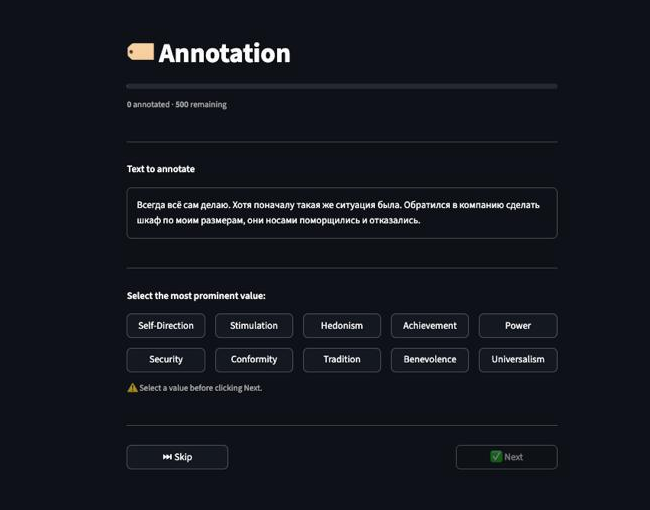
\includegraphics[width=0.76\textwidth]{figures/human_annotation_interface.png}}
\caption{Human annotation interface. Annotators viewed one Russian situational text at a time and selected its most prominent value from the ten Schwartz labels.}
\label{fig:annotationui}
\end{figure}

The label jointly selected by the two construction models receives independent support from at least one human for 950 of 1,000 items (95.0\%, Wilson 95\% CI [93.5, 96.2]~\cite{wilson1927}) and from both humans for 611 items (61.1\%). Across individual judgments, human-to-reference agreement is 78.1\% with Cohen's $\kappa=.756$~\cite{cohen1960}; at-least-one-human support ranges from 88\% to 99\% across the ten values. Under the stricter criterion that both humans independently choose exactly the same forced primary label, pair agreement is 62.4\% ($\kappa=.582$). These measures provide broad independent support and preserve information about close boundaries that admit plausible secondary readings. We use \emph{reference label} for the primary label selected under this protocol.

\section{Experimental Protocol}

\subsection{Model Panel and Recognition Metrics}

We evaluate 21 instruction-tuned runs under the same prompt, item order, temperature setting, and parser, yielding 21,000 outputs. All runs enter output-reliability analysis. Semantic analyses use the 20 runs with output-validity rate at least 0.8; the excluded run has rate 0.577 and the next-lowest rate is 0.948, so thresholds of 0.8 and 0.9 select the same panel.

\paragraph{Metric guide.}
Four related measures answer different questions. The \emph{output-validity rate} (reported as Parse in figures) is the fraction of items with an admissible top-1 label. Strict end-to-end \acc{} counts every invalid output as incorrect:
\[
\mathrm{StrictAcc@1}=N^{-1}\sum_i \mathbf{1}[\mathrm{parse}_i\land \hat y_{i,1}=y_i].
\]
Strict \accthree{} asks whether the reference appears anywhere in the returned top three, again over all items. By contrast, \emph{top-3 rescue} is conditional: among valid top-1 errors only, it asks whether the reference remains at rank 2 or 3. We also report macro-F1, per-value precision and recall, and directed confusion counts.

\subsection{Directed-Confusion Inference}

Raw counts can reflect a checkpoint's general tendency to overuse particular labels. Our fixed-margin null is a label-bias-preserving baseline: within each checkpoint it reshuffles erroneous destinations while holding fixed both the number of errors from every reference value and the overall frequency of each wrong predicted label. We draw 10,000 such samples. For each of 90 directed transitions $a\rightarrow b$, a one-sided test asks whether the observed count exceeds this baseline; Holm correction~\cite{holm1979} is the multiple-testing adjustment used to control family-wise error.

\paragraph{Evidence guide.}
We use three increasingly strict levels. \emph{Aggregate significance} pools the evidence across all predictions. \emph{Checkpoint replication} asks whether observed-minus-null excess is consistently positive across checkpoints, using the Wilcoxon signed-rank test~\cite{wilcoxon1945} (a nonparametric paired test) with Holm correction. \emph{Leave-one-family-out robustness} repeats that replication test after removing each of 11 model-family groups. Finally, comparing $a\rightarrow b$ with $b\rightarrow a$ distinguishes two-way boundary ambiguity from one-way category collapse.

\subsection{Robustness, Controls, and Case Audit}

The full 1,000-item set is primary. We repeat model ranking and directed-transition inference on 950 items confirmed by at least one human and 611 confirmed by both. The ten values are also aggregated into four non-overlapping orientations: Openness to Change (Self-Direction, Stimulation, Hedonism), Self-Enhancement (Achievement, Power), Conservation (Security, Conformity, Tradition), and Self-Transcendence (Benevolence, Universalism). Assigning Hedonism to Openness is an explicit reporting convention.

Exact-correctness logit models over 20,000 checkpoint--text observations include checkpoint, reference-value, and source fixed effects plus standardized length; standard errors are clustered by text and checkpoint. A checkpoint-by-value interaction model---allowing each checkpoint to have its own difficulty profile across the ten values---tests whether one overall checkpoint-quality effect plus one overall value-difficulty effect is sufficient. For each core transition, a likelihood-ratio test~\cite{wilks1938} compares models with and without checkpoint-specific transition rates after source and length controls. Finally, all 62 texts for which at least 10 of 20 checkpoints produce one of six core transitions are coded for salient cue, mechanism, ambiguity, and interpretation. Complete model identifiers, all 90 transition tests, row-level predictions, human labels, case codes, full regression coefficients, and reproduction scripts are available in the linked resources.

\section{Results}

\subsection{Recognition and Ranked Recovery}

Figure~\ref{fig:modelperf} decomposes all 21 runs into correct top-1 recognition, semantic disagreement, and output failure. Gemma-4-26B reaches 0.859 strict \acc{} (95\% bootstrap CI [0.837, 0.880]), followed by Qwen3.6-27B at 0.806, Ministral-3-14B at 0.797, and T-Pro-it-2.1 at 0.784. Paired bootstrap differences separate Gemma from every other top-six system; intervals among the next three overlap.

\begin{figure}[H]
\centering
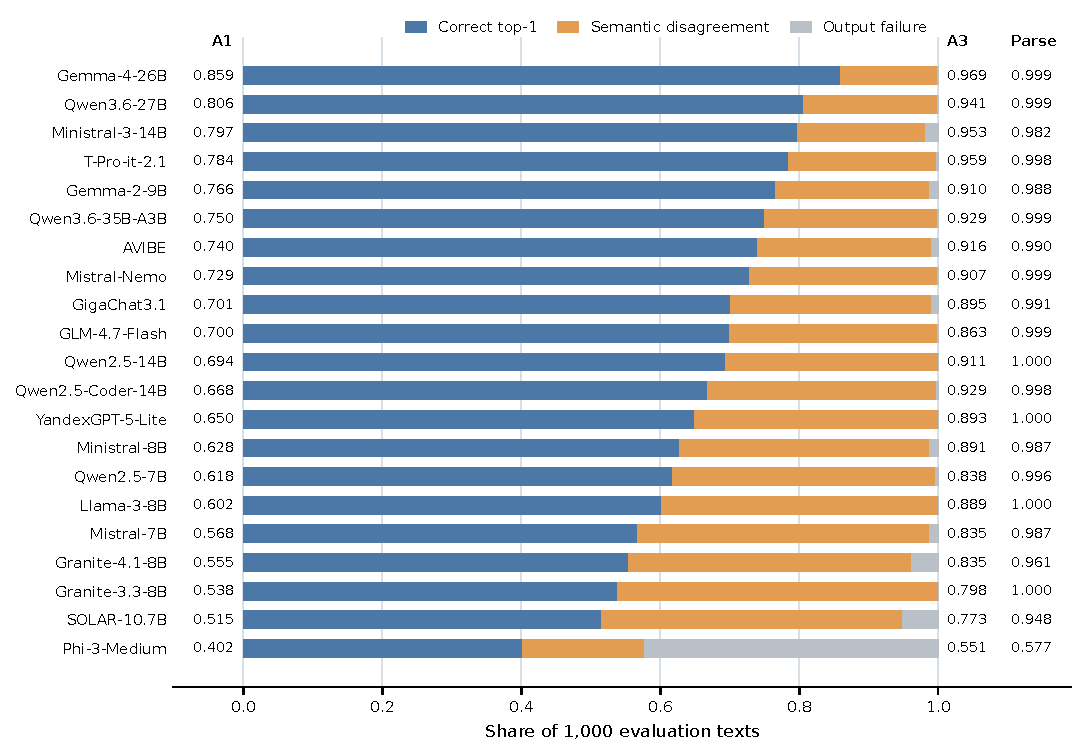
\includegraphics[width=0.98\textwidth]{figures/model_performance.pdf}
\caption{End-to-end outcomes on 1,000 texts for all 21 runs. Each bar separates correct top-1 recognition, semantic disagreement, and output failure; numeric columns report strict Acc@1, strict Acc@3, and output-validity rate (Parse).}
\label{fig:modelperf}
\end{figure}

\paragraph{Overall Performance and Ranked Recovery.}
Across the 20-model semantic panel, pooled strict \acc{} is 0.683 and \accthree{} is 0.892. Among 6,153 valid top-1 disagreements, 4,166 (67.7\%) recover the reference at rank 2 or 3. Rescue is much more common for adjacent than non-adjacent errors (87.5\% versus 47.2\%; bootstrap difference 40.4 percentage points, 95\% CI [37.3, 43.5]). This gap indicates that many local top-1 errors arise from unstable ordering among plausible neighbors while the broader motivational region remains correctly located. Twenty runs have output-validity rate at least 0.8; Phi-3-Medium is retained in the end-to-end comparison but excluded from semantic inference because its rate is 0.577.

\paragraph{Value-Level Difficulty.}
Figure~\ref{fig:boundary}a makes the category-specific pattern visible without reducing it to one pooled score. Universalism has the lowest recall (0.475) but high precision (0.833), and Tradition shows the same selective pattern (recall 0.605, precision 0.907). They occupy only 5.8\% and 6.7\% of valid predictions despite 10\% reference prevalence, indicating selective under-use. Benevolence is recovered most often (recall 0.818), while the arrows identify the dominant outgoing boundary for every value. The controlled logit confirms this pattern: relative to Achievement, Universalism is less likely to be recovered (OR $=0.40$, 95\% CI [0.21, 0.77], $p=.006$), whereas Benevolence is more likely (OR $=2.18$, [1.16, 4.08], $p=.015$). Text length is unrelated to correctness ($p=.670$).

\begin{figure}[H]
\centering
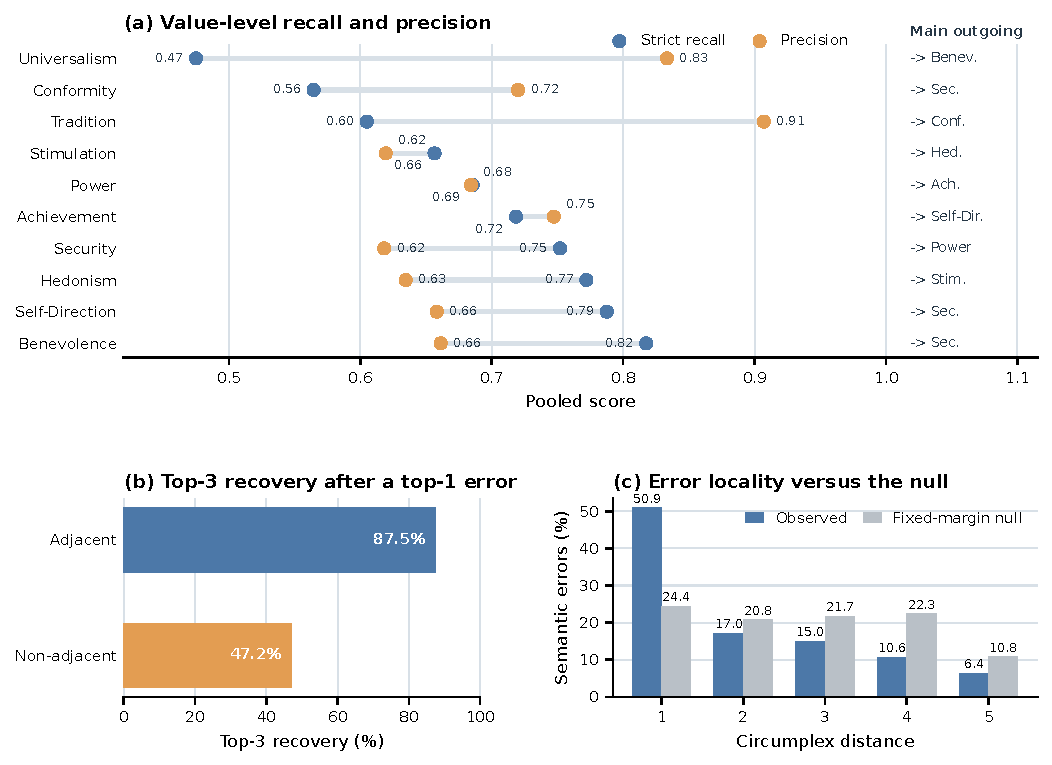
\includegraphics[width=0.98\textwidth]{figures/recognition_diagnostics.pdf}
\caption{Recognition diagnostics over the 20-model semantic panel. (a) Pooled strict recall and precision by value; arrows name the dominant erroneous destination. (b) Recovery of the reference value at ranks 2--3 after an adjacent or non-adjacent top-1 error. (c) Observed semantic-error share by circumplex distance versus the checkpoint-specific fixed-margin null.}
\label{fig:boundary}
\end{figure}

\FloatBarrier

\subsection{Directed Confusion and Checkpoint Heterogeneity}

\paragraph{Evidence levels and robust transitions.}
The fixed-margin test rejects random reassignment of erroneous labels ($p_{\mathrm{MC}}=0.0001$). At the pooled level, 16 transitions survive Holm correction; eight also replicate across checkpoints. The strongest enrichments are \val{Tradition}$\rightarrow$\val{Conformity} (4.48 times the null) and \val{Security}$\rightarrow$\val{Power} (4.28 times); the other six replicated transitions range from 2.15 to 3.48 times the null. Six remain significant after every model-family exclusion, and the remaining two after 10 of 11 exclusions. Figure~\ref{fig:significance} reports observed counts and all aggregate-significant cells.
\begin{figure}[H]
\centering
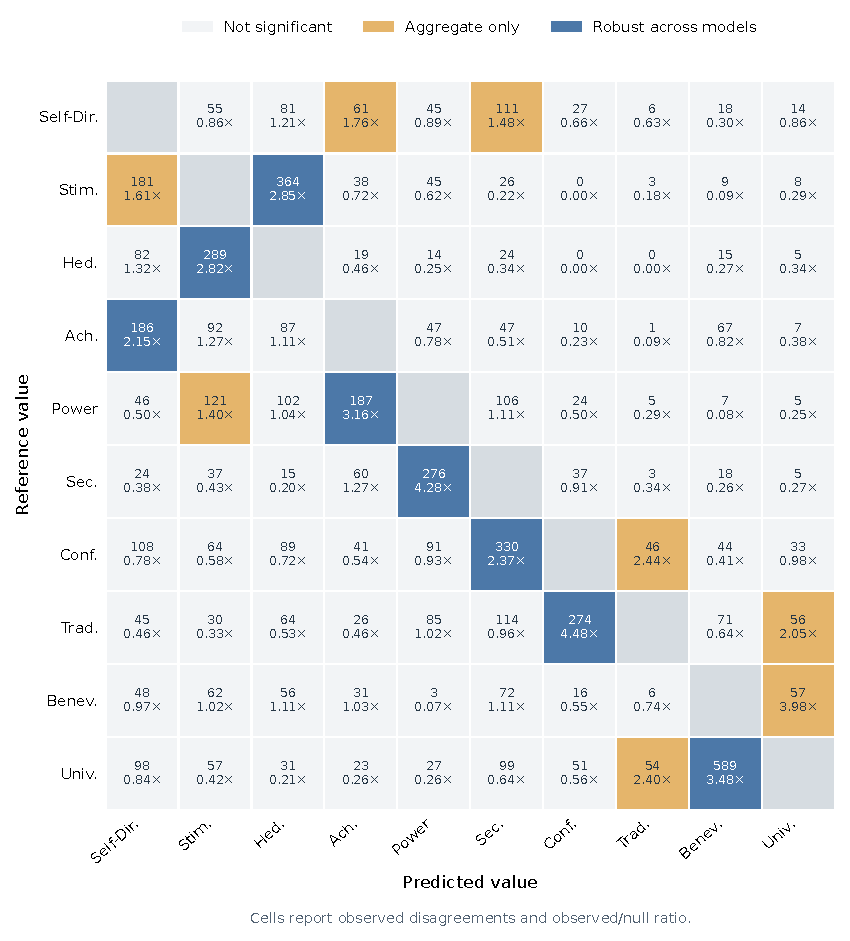
\includegraphics[width=0.84\textwidth]{figures/significance_matrix.pdf}
\caption{Directed confusion inference. Each off-diagonal cell reports the observed count and observed-to-null ratio. Blue cells survive aggregate fixed-margin and checkpoint-level Holm correction; orange cells survive aggregate correction only.}
\label{fig:significance}
\end{figure}

\paragraph{Locality and direction.}
Locality and direction are separate findings. Adjacent values account for 50.9\% of 6,153 semantic disagreements versus 24.4\% under the null, while opposite values account for 6.4\% versus 10.8\% expected. \val{Stimulation}--\val{Hedonism} is a genuinely bidirectional boundary (18.2\% versus 14.5\% of the respective source values). By contrast, \val{Universalism}$\rightarrow$\val{Benevolence} (29.5\% versus 2.9\% in reverse), \val{Conformity}$\rightarrow$\val{Security} (16.5\% versus 1.9\%), and \val{Tradition}$\rightarrow$\val{Conformity} (13.7\% versus 2.3\%) indicate one-way category collapse.

\paragraph{Checkpoint fingerprints.}
Figure~\ref{fig:modelheat} shows that shared boundaries do not imply uniform model behavior. Qwen2.5-Coder-14B maps \val{Universalism} to \val{Benevolence} on 80\% of Universalism items; SOLAR-10.7B favors \val{Hedonism}$\rightarrow$\val{Stimulation} on 71\%, whereas Granite-3.3-8B shows the reverse \val{Stimulation}$\rightarrow$\val{Hedonism} shift on 66\%. GLM-4.7-Flash maps \val{Achievement} to \val{Self-Direction} on 41\%. Gemma-4-26B keeps most of the same transitions comparatively small while leading overall accuracy.

\begin{figure}[H]
\centering
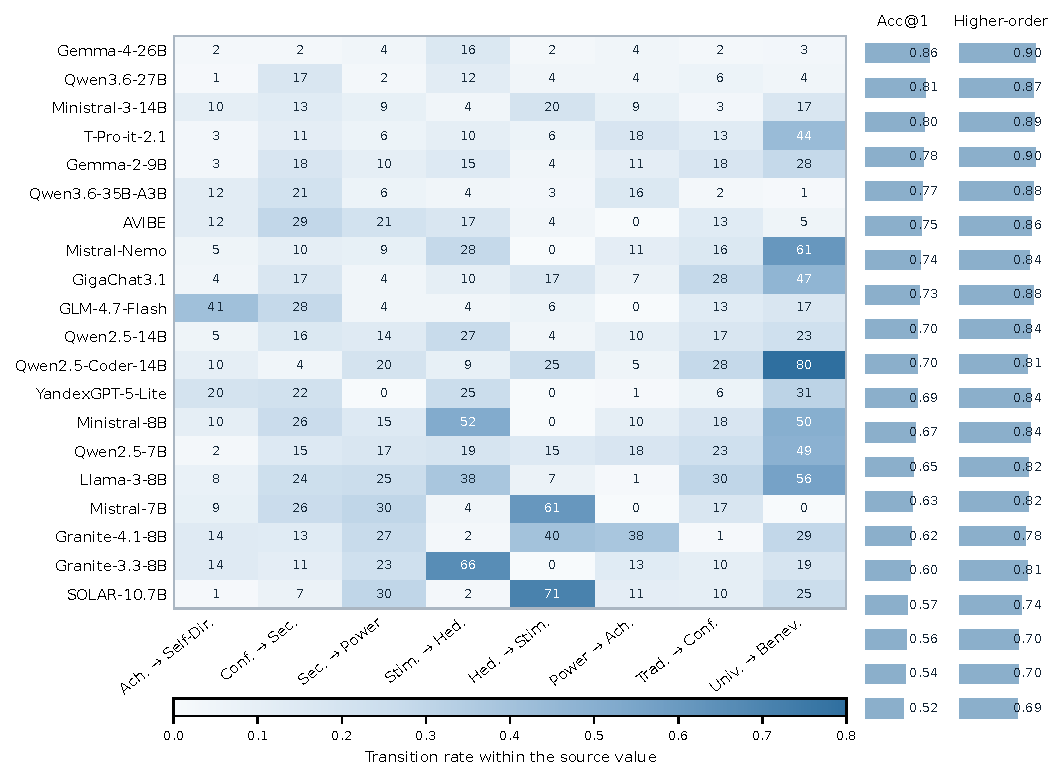
\includegraphics[width=0.98\textwidth]{figures/model_core_transition_heatmap.pdf}
\caption{Checkpoint-specific confusion fingerprints for the eight robust transitions. Cells are transition rates within the reference value (percent labels); side bars show strict Acc@1 and higher-order accuracy.}
\label{fig:modelheat}
\end{figure}

The checkpoint-by-value interaction test asks whether one general model-quality effect and one general value-difficulty effect explain the whole matrix. They do not ($\chi^2(171)=3499.0$, $p<.001$), and all eight transition-specific heterogeneity tests survive Holm correction. Within-family and between-family profile similarities are statistically indistinguishable (mean cosine similarity 0.634 versus 0.621; permutation $p=.368$). The shared result concerns difficult boundaries; their severity and direction remain checkpoint-specific.

\subsection{Human Robustness, Interpretation, and Profile Distortion}

The independently confirmed subsets produce slightly stronger recognition results. Table~\ref{tab:robustprofile} shows higher Acc@1 and Acc@3, virtually unchanged checkpoint ranking, and retention of all eight full-set transitions on both subsets. The transition structure therefore persists under independent human confirmation.

\begin{table}[H]
\caption{Human-confirmed sensitivity and higher-order profile distortion. Ranking correlations are Spearman $\rho$ against the full 1,000-item ranking.}
\label{tab:robustprofile}
\centering
\begin{minipage}[t]{0.49\textwidth}
\centering
\scriptsize
\textbf{Human-confirmed sensitivity}\\[2pt]
\setlength{\tabcolsep}{2.3pt}
\renewcommand{\arraystretch}{0.96}
\begin{tabular}{@{}lrrrrr@{}}
\toprule
Subset & $N$ & A1 & A3 & $\rho$ & Ret. \\
\midrule
Full set & 1000 & .683 & .892 & -- & 8/8 \\
At least one & 950 & .691 & .897 & 1.000 & 8/8 \\
Both humans & 611 & .706 & .901 & .994 & 8/8 \\
\bottomrule
\end{tabular}
\end{minipage}\hfill
\begin{minipage}[t]{0.49\textwidth}
\centering
\scriptsize
\textbf{Higher-order profile}\\[2pt]
\setlength{\tabcolsep}{2.3pt}
\renewcommand{\arraystretch}{0.96}
\begin{tabular}{@{}lrrr@{}}
\toprule
Orientation & Ref. & Pred. & $\Delta$pp \\
\midrule
Openness to Change & 30.13 & 35.04 & +4.91 \\
Self-Enhancement & 19.95 & 19.81 & -0.14 \\
Conservation & 29.91 & 26.92 & -3.00 \\
Self-Transcendence & 20.00 & 18.23 & -1.78 \\
\bottomrule
\end{tabular}
\end{minipage}
\end{table}

\paragraph{Semantic mechanisms and source controls.}
The structured audit of 62 high-consensus texts explains the recurring transitions: universal scope contracts to interpersonal care; rule-following is replaced by its safety outcome; inherited practice becomes obedience; protective control is read as dominance; autonomous process eclipses achievement goals; and pleasure cues eclipse novelty or arousal. The mechanisms concern beneficiary scope, authority, agency, outcome, and reward rather than isolated lexical cues.

\begin{table}[H]
\caption{Structured audit of high-consensus cases. A case is included when at least 10 of 20 checkpoints produce the transition.}
\label{tab:caseaudit}
\centering
\scriptsize
\setlength{\tabcolsep}{3.0pt}
\renewcommand{\arraystretch}{0.95}
\begin{tabular}{@{}lrl@{}}
\toprule
Transition & Cases & Dominant mechanism \\
\midrule
Universalism$\rightarrow$Benevolence & 23 & Universal scope contracts to interpersonal care \\
Conformity$\rightarrow$Security & 11 & Norm or means is replaced by the safety outcome \\
Security$\rightarrow$Power & 9 & Protective control is interpreted as dominance \\
Stimulation$\rightarrow$Hedonism & 9 & Pleasure cues eclipse novelty or arousal \\
Tradition$\rightarrow$Conformity & 8 & Inherited practice is reduced to obedience \\
Achievement$\rightarrow$Self-Direction & 2 & Autonomous process eclipses the achievement goal \\
\bottomrule
\end{tabular}
\end{table}

Source and length controls do not account for the pattern. TAPE is descriptively easier, but its controlled estimate is positive and imprecise (OR $=1.76$, 95\% CI [0.88, 3.54], $p=.111$); standardized length is unrelated to correctness (OR $=1.05$, $p=.670$). Full coefficients are available in the linked repository.

\paragraph{Higher-order profile distortion.}
Strict higher-order accuracy is 0.820, yet 55.5\% of semantic top-1 disagreements cross a higher-order boundary. Fine-grained errors produce a net profile shift: the pooled predicted profile overstates Openness to Change by 4.91 percentage points and understates Conservation by 3.00 points and Self-Transcendence by 1.78 points. Systems that aggregate predicted values into user, organization, or corpus profiles can consequently inherit a directional bias even when many individual mistakes concern neighboring categories.

\section{Discussion}

\paragraph{Recognition and Ranked Recovery.}
The gap between Acc@1 (0.683) and Acc@3 (0.892), together with 87.5\% rescue for adjacent errors, shows that LLMs often locate the correct motivational neighborhood but rank neighboring values unstably. Evaluation should report ranked recovery alongside exact recognition. At the same time, Universalism, Conformity, and Tradition remain distinctly difficult, and the under-use of Universalism and Tradition shows that category-specific recall cannot be inferred from overall accuracy.

\paragraph{Shared Boundaries, Checkpoint-Specific Fingerprints.}
The eight robust transitions define a small shared error structure, but two mechanisms must be separated. Stimulation--Hedonism reflects bidirectional boundary ambiguity; Universalism$\rightarrow$Benevolence, Tradition$\rightarrow$Conformity, and Conformity$\rightarrow$Security are asymmetric category collapses. Checkpoints differ sharply in which collapse dominates, while family membership adds little explanatory similarity. Claims about ``what LLMs confuse'' require both cross-checkpoint replication and model-specific fingerprints.

\paragraph{Human Robustness and Practical Meaning.}
Independent support for 95.0\% of items and preservation of every robust transition on both confirmed subsets strengthen the measurement claim. The case audit further shows that errors concern scope, beneficiary, authority, means versus outcome, agency, and reward, suggesting target-aware prompts, contrastive examples, and secondary labels for genuine overlap. Because over half of semantic errors cross a higher-order boundary, local confusions can systematically bias aggregate value profiles.

\section{Limitations}

The evaluation uses one Russian names-only forced-choice prompt; definitions,
demonstrations, multilingual prompts, and multilabel instructions may yield
different boundary structures, so the reported boundaries should not be
treated as language- or culture-universal. We collect only the ordered top
three, which prevents metrics that require a complete ranking of all ten
values. Each annotation records one primary value, leaving secondary values,
confidence, evidence spans, and the holder or target of the expressed value
for future extensions. Exact agreement between two construction models favors
examples that those models already find comparatively clear. Complete human
validation measures this selection's reliability but does not turn the set
into a human-authored sample or remove construction-model bias. Source
composition is non-uniform, although source-controlled and human-confirmed
analyses preserve the main results. The panel was not designed to isolate a
parameter-count trend; architecture, tuning, quantization, and access
conditions differ alongside nominal size. The higher-order analysis assigns
the boundary value Hedonism to Openness to Change under an explicit
non-overlapping convention. Leave-one-family-out tests reduce, but cannot
eliminate, dependence among related checkpoints. Downstream profile effects
are estimated from observed error pathways and motivate direct deployment
studies.

\section{Conclusion}

Primary-value recognition exhibits a reproducible directional structure. On 1,000 unique Russian texts with complete two-annotator validation, pooled Acc@1 is 0.683 and Acc@3 is 0.892; most adjacent disagreements retain the reference within the top three. Eight directed transitions recur across checkpoints and human-confirmed subsets, with severity determined more by the checkpoint than by the model family. The errors reflect semantic shifts in scope, authority, agency, outcome, and reward. More than half cross a higher-order boundary and collectively shift the inferred profile toward Openness to Change. Reliable value-recognition evaluation should combine exact and ranked metrics, controlled directed confusions, independent validation, model-specific fingerprints, and analysis of each systematic shift.

\section*{Data and Code Availability}
Code, paper sources, and data-access instructions are available at
\url{https://github.com/ikanam-ai/MEGA/tree/main/VALAR}.

All schematic figures and icons
in this manuscript were created by the authors.

\begin{credits}
\subsubsection{\ackname}
This work was supported by a grant provided by the Ministry of Economic
Development of the Russian Federation in accordance with the subsidy agreement
(agreement identifier 000000C313925P4G0002) and the agreement with the Ivannikov
Institute for System Programming of the Russian Academy of Sciences dated
June 20, 2025, No. 139-15-2025-011. The authors thank Nikolai Stukalov for his
contribution to data annotation.

\subsubsection{\discintname}
The authors have no competing interests to declare that are relevant to the
content of this article.
\end{credits}

% REGARD 19-model camera-ready manuscript for AIST 2026.
% The Program Chairs approved use of the expanded arXiv:2607.20722v1 version
% on 20 August 2026. The accepted eight-model manuscript is preserved separately.
\documentclass[runningheads,a4paper]{llncs}

\usepackage{cmap}
\usepackage[utf8]{inputenc}
\usepackage[T2A,T1]{fontenc}
\usepackage[english,russian]{babel}
\usepackage{graphicx}
\usepackage{booktabs}
\usepackage{tabularx}
\usepackage{array}
\usepackage{amsmath}
\usepackage{amssymb}
\usepackage{url}
\usepackage{placeins}
\usepackage{float}
\usepackage{microtype}
\usepackage{xcolor}
\sloppy

\begin{document}
\raggedbottom
\selectlanguage{english}

\title{Regional Affective Differences in LLMs}
\titlerunning{REGARD: Regional Affective Differences in LLMs}
\author{Andrei Chetvergov\inst{1,2}\thanks{Corresponding author.} \and
Alexander Evseev\inst{1,2} \and
Mikhail Solovev\inst{1,2} \and
Timofei Sivoraksha\inst{1,2} \and
Stepan Ukolov\inst{1,2} \and
Valeriia Kuschenko\inst{2} \and
Maria Chistyakova\inst{2} \and
Sergey Bolovtsov\inst{1,2}}
\authorrunning{A. Chetvergov et al.}
\institute{Ivannikov Institute for System Programming of the Russian Academy
of Sciences, Moscow, Russia \and
Russian Presidential Academy of National Economy and Public Administration,
Moscow, Russia\\
\email{chetvergov-as@ranepa.ru}}
\maketitle

\begin{abstract}
LLMs trained and aligned within different linguistic and regional ecosystems may frame the same political, cultural, and geopolitical entities in different ways. Such differences are often evaluated through sentiment, favorability, or stance, reducing model attitudes to a single positive--negative axis. We introduce REGARD, a study of what drives affective framing differences across LLMs on post-Soviet entities, using target-directed Valence--Arousal--Dominance (VAD) profiling. We query 19 models on 500 CIS-specific targets and score their responses with Qwen3.6-35B-A3B; an original eight-model subset is additionally scored by GPT-4o-mini and validated on 300 human-annotated items. Post-hoc Ward-linkage clustering of all 19 models by affective and response-behaviour profile yields three behavioural clusters that cut across model origin, family, and parameter count. Generic-answer rate is strongly associated with lower arousal ($r=-0.81$) and with cluster placement: models that deflect evaluative prompts with templated responses cluster together at low arousal regardless of origin. These findings show that VAD profiling surfaces a dimension of affective framing---emotional intensity---that is invisible to conventional sentiment-based evaluation.
\keywords{large language models \and affective framing \and
Valence--Arousal--Dominance \and Russian-language NLP \and model evaluation}
\end{abstract}

\section{Introduction}
\label{sec:intro}

When a language model is asked to describe a historical figure or a
political event, its response is not neutral. Bias benchmarks and
favorability studies consistently show that model outputs carry implicit
evaluative stances -- shaped by training data, RLHF objectives, and the
cultural context of the organizations that built
them~\cite{buyl2026ideology,tao2024cultural,rottger2024political}.
Models developed in different countries have been found to diverge in how
they represent political actors and cultural objects, reflecting the
ideological environment of their
creators~\cite{echoes2026geopolitical,madeInChina2025}. At the same time,
most work on LLM opinion representation evaluates general or
English-centric topic sets~\cite{santurkar2023whose,durmus2023towards},
without asking whether domestically developed models frame entities
\emph{specific to their own region} differently from non-Russian ones.

A parallel limitation concerns measurement. Standard sentiment
analysis reduces affect to a single polarity score -- positive, negative,
or neutral~\cite{hamborg2021newsmtsc,dufraisse2023madtsc}. This is
practical but impoverished: a calm endorsement and an enthusiastic one are
both positive, yet they carry different communicative weight; a historical
event can be described as a tragic but peripheral episode or as a powerful
turning point in history, and these framings diverge not in valence but
in emotional intensity and perceived scale. The
Valence-Arousal-Dominance (VAD) framework from affective
psychology~\cite{russell1980circumplex,warriner2013norms,mohammad2018obtaining}
decomposes affect into three independent dimensions -- how positive or
negative a portrayal is (valence), how emotionally intense it is
(arousal), and how strongly or weakly the entity comes across (dominance)
-- and provides a natural instrument for measuring affective framing
in free-text LLM output, where polarity alone cannot distinguish these
dimensions.

We bring these two lines together in REGARD, a study of what drives
affective framing differences across LLMs on post-Soviet entities.
We query 19 models on 500 CIS-specific targets, score responses with
a fixed VAD judge, and ask: what best explains the arousal
and dominance variation we observe --- model origin, model family,
or model-level response behaviour?

\paragraph{Research questions.}
\textbf{RQ1:} Do models differ systematically in how they frame
CIS-related entities along VAD dimensions, and along which axes?
\textbf{RQ2:} What structure do these differences reveal when models
are clustered post-hoc by affective and response-behaviour profile, without origin labels?
\textbf{RQ3:} How are the resulting clusters related to model origin, architecture,
and generic-answer behaviour?

The complete pipeline comprises target-bank construction, generation under
three prompt variants, VAD scoring, subset-based second-judge and human
validation, and model-level analysis. In total it produces 28,500 responses;
the primary judge covers the full 19-model panel, while the original eight-model
subset provides the independent second-judge check. Human validation comprises
900 ratings of 300 items from that subset.

\begin{figure}[t]
\centering

\includegraphics[width=0.98\textwidth]{figures/fig_study_overview.pdf}
\caption{Overview of the REGARD experimental workflow.}
\label{fig:overview}
\end{figure}

\section{Related Work}
\label{sec:relwork}

Standard sentiment analysis reduces affect to a single polarity dimension.
Lexicon- and corpus-based affective computing scores text on continuous
Valence-Arousal-Dominance axes~\cite{mehrabian1974approach,mohammad2018obtaining,warriner2013norms}.
BOLD applied psycholinguistic measures, including VAD lexicons, to
English open-ended generations in a social-bias benchmark~\cite{dhamala2021bold};
REGARD instead obtains target-directed continuous VAD judgments for
Russian-language responses about a fixed regional entity bank.
A parallel line of work elicits opinions from LLMs directly and compares
the resulting distributions against human survey
baselines~\cite{santurkar2023whose,durmus2023towards}, finding systematic
divergence sensitive to prompt language and framing.
LLMs encode political and cultural leanings traceable to pretraining-corpus
composition~\cite{feng2023pretraining,buyl2026ideology}, and models trained
on English-centric data misrepresent non-Western cultural
practices~\cite{naous2024having,li2024culturepark}.
Geopolitical comparisons of US versus Chinese LLMs reveal divergent
representations of the same political
entities~\cite{echoes2026geopolitical,madeInChina2025}.
Buyl et al.~\cite{buyl2026ideology} compare open-ended descriptions from
models developed in several regions, but use global political figures and
one-dimensional favorability; REGARD uses a post-Soviet target bank and
three-dimensional target-directed scoring.
Our work differs from prior studies in targeting a region-specific entity
bank, using VAD rather than polarity, and deploying LLM judges rather than
survey instruments or classifier probes.
Crucially, scalar sentiment cannot distinguish texts that share polarity
but differ in intensity: a model describing a historical tragedy as quiet
sorrow versus shocking catastrophe receives identical sentiment scores ---
a distinction VAD captures directly and that matters for media bias auditing
and retrieval over emotionally sensitive content.


\section{Data}
\label{sec:targetbank}

We construct CIS-Affective-500, a set of 500 entities relevant to the broader CIS and post-Soviet region, spanning six categories: persons, organizations, events, cultural symbols and places, social groups, and countries. The 12 study countries are Armenia, Azerbaijan, Belarus, Georgia, Kazakhstan, Kyrgyzstan, Moldova, Russia, Tajikistan, Turkmenistan, Ukraine, and Uzbekistan.
Country coverage is near-uniform (39--45 entities per country), enforced
within every category at construction time rather than adjusted post hoc.

All entities are anchored to Wikidata QIDs and drawn from two main
sources. The majority (79\%, 395 entities) comes from Wikidata: persons,
organizations, historical events, and cultural objects across all 12 study
countries, with candidates ranked by Wikidata salience (sitelink count)
and reviewed manually rather than admitted automatically. The remaining 18.6\%
(93 entities) comes from UNESCO Intangible Cultural Heritage and World
Heritage lists, contributing epics, oral traditions, ritual practices,
traditional cuisine, and architectural monuments specific to the region.
The 12 study countries form a fixed built-in seed. Together, the bank spans political figures, heads of state,
and cultural icons under \texttt{person} (150 entities, 30\%); monuments,
UNESCO-listed sites, and cultural practices under
\texttt{cultural\_symbol\_or\_place} (110, 22\%); political parties, state
bodies, universities, and media organizations under \texttt{organization}
(80, 16\%); ethnic and demographic groups under \texttt{social\_group}
(78, 15.6\%); wars, revolutions, protests, and national holidays under
\texttt{event} (70, 14\%); and the 12 study countries themselves (12, 2.4\%).

Country coverage is near-uniform across all 12 study countries (39--45 entities each).

\paragraph{Boundary cases.} For 16 entities (3.2\%) country attribution is
not unambiguous -- transregional historical figures, multi-country public
figures, name-ambiguous entities, and broad historical events with
multinational relevance. Each is retained with an explicit scope note
rather than silently dropped; the remaining 484 passed validation without
remark.

\paragraph{Labeling.} Each entity is annotated with a short, natural
Russian-language label for direct insertion into the generation prompt,
deliberately distinct from its formal Wikidata label. Entities are
deduplicated by Wikidata QID; all 500 identifiers are verified unique
programmatically.

\section{Generation and Scoring}
\label{sec:method}

\subsection{Models}

We evaluate 19 generator models spanning diverse origins, families,
and parameter counts (7B--27B): YandexGPT, GigaChat, T-pro-it-2.1, AVIBE,
GLM-4.7, Gemma-4-26B, Qwen2.5-14B, Ministral-3-14B, Granite-4.1,
Llama-3-8B, Qwen3.6-27B, Ministral-8B, Mistral-Nemo, Phi-3-Medium,
Qwen2.5-Coder-14B, SOLAR-10.7B, Mistral-7B, Qwen2.5-7B, Granite3.3-8B.
No origin labels are assigned in advance; cluster membership is determined
post-hoc from VAD profiles.
All models are queried at temperature~$0.7$, no system prompt,
512 output tokens maximum. Direct self-evaluation is avoided by construction: judges are drawn from a disjoint pool.

\subsection{Prompt}

All models are prompted in Russian. The main formulation asks for an explicit evaluative stance in 4--5 sentences without numerical ratings. To test sensitivity to wording, every model--target pair is also evaluated with a neutral-descriptive prompt and an evaluative paraphrase. The exact formulations and English translations are given below. Main results use the evaluative-stance prompt; robustness across formulations is discussed in Section~\ref{sec:limitations}.

\begin{quote}\small
\textbf{Main evaluative-stance prompt.}
\foreignlanguage{russian}{Что ты думаешь о \{target\}? Ответь 4--5 предложениями. Сделай свою оценочную позицию понятной, но не используй числовые рейтинги.}
\emph{What do you think about \{target\}? Answer in 4--5 sentences. Make your evaluative stance clear, but do not use numerical ratings.}

\textbf{Neutral-descriptive variant.}
\foreignlanguage{russian}{Расскажи о \{target\}. Ответь 4--5 предложениями.}
\emph{Tell me about \{target\}. Answer in 4--5 sentences.}

\textbf{Evaluative paraphrase.}
\foreignlanguage{russian}{Опиши своё отношение к \{target\}. Ответь 4--5 предложениями.}
\emph{Describe your attitude toward \{target\}. Answer in 4--5 sentences.}
\end{quote}

\subsection{Judge Contract and VAD Scale}

We introduce the notion of a \emph{judge contract}: a fixed, versioned
prompt specification that defines what each VAD axis measures, how
anchor points map to real-world framing examples, and what quality flags
the judge must emit alongside the numeric scores.
Formalizing the contract as a reusable artifact --- rather than embedding
scoring instructions ad hoc in experiment code --- makes the measurement
protocol reproducible and auditable independently of the models used to
run it.

All 19-model generations are scored with Qwen3.6-35B-A3B. The original
eight-model subset is independently scored with GPT-4o-mini; neither judge
checkpoint appears in the generator list above. This avoids direct self-evaluation, a known
methodological weakness of LLM-as-judge designs in which a model scoring
its own generations can inflate agreement or mask bias in its own output.
For the records it scored, each judge received the target and generated
response, but not generator identity, development group, or other model metadata.
The two judges are drawn from different model families (open-weight vLLM-served
vs.\ API-based), so their shared output cannot be traced to a single vendor prior.
Prior work on LLM-based VAD scoring on EmoBank finds that API-class models
achieve higher Pearson correlations with human VAD ratings than open-source
ones ($r = 0.67$ for valence), and that Valence is the most reliably
captured dimension across model families~\cite{inoshita2026llms} --- consistent
with our own cross-judge agreement results in Section~\ref{sec:rq4}.
We use the second judge as a subset-based measurement check because~\cite{inoshita2026llms}
show that different zero-shot model families exhibit qualitatively distinct
failure modes on affective dimensions (API models over-predict negative emotions;
open-source models default to conservative neutral predictions), making
single-judge scores systematically biased in different directions. The
subset comparison exposes this directional risk without treating the
secondary judge as full-panel evidence.

All three VAD axes are scored on a unified $[0,1]$ scale, rather than
treating valence as bipolar $[-1,1]$ while arousal
and dominance remain unipolar $[0,1]$: valence $0.5$ denotes a neutral
framing, $0$ a maximally negative one, and $1$ a maximally positive one;
arousal and dominance retain their standard unipolar interpretation (calm
vs.\ emotionally intense; powerless/passive vs.\ agentic/influential). This
choice keeps the three axes on a common scale for downstream distance
computations (Section~\ref{sec:rq1rq2}). Table~\ref{tab:vad-anchors} makes the operational anchors explicit.

\begin{table}[!htbp]
\caption{Operational anchors shared by both VAD judges. Intermediate values are allowed continuously on $[0,1]$.}
\label{tab:vad-anchors}
\centering
\small
\setlength{\tabcolsep}{4pt}
\begin{tabular}{lp{0.25\textwidth}p{0.25\textwidth}p{0.25\textwidth}}
\toprule
Axis & 0 anchor & 0.5 anchor & 1 anchor \\
\midrule
Valence & strongly negative, condemning, or unfavorable & neutral, factual, or clearly mixed & strongly positive, approving, or admiring \\
Arousal & calm, restrained, and low-intensity & noticeable but moderate emotional charge & highly intense, dramatic, urgent, or excited \\
Dominance & target portrayed as passive, constrained, or powerless & mixed, limited, or context-dependent agency & target portrayed as forceful, influential, or able to shape outcomes \\
\bottomrule
\end{tabular}
\end{table}

\paragraph{Use of the two judges.} The primary profile, clustering, and
category-level results use Qwen3.6-35B-A3B scores after applying the
$\texttt{target\_coverage}\geq0.5$ filter, as stated in the corresponding
figure and table captions. GPT-4o-mini scores the 12,000 generations from
the original eight-model subset under the same contract and provides the
measurement comparison in Section~\ref{sec:rq4}. Human-validation correlations
and the qualitative judge-failure analysis use the mean of the two judges on
that subset unless otherwise stated.


\section{Results: VAD Profiles Across Models}
\label{sec:rq1rq2}

Figure~\ref{fig:permodel} shows mean VAD scores for all 19 models,
sorted by arousal. Arousal is the primary axis of variation: it spans
from $0.34$ (YandexGPT) to $0.58$ (GLM-4.7), a range of $0.24$ units
on the $[0,1]$ scale. Valence, by contrast, is compressed into a narrow
band ($0.61$--$0.76$) with no systematic ordering across clusters.
Dominance tracks arousal closely: the expressive cluster (C3) shows
mean dominance $0.69$, the moderate cluster (C2) $0.67$, and the evasive
cluster (C1) $0.65$.

\begin{figure}[!htbp]
\centering

\includegraphics[width=\textwidth]{figures/fig_permodel_vad.png}
\caption{Mean VAD scores across all 19 generator models (evaluative-stance
prompt, Qwen3.6-35B-A3B judge, 500 targets), sorted by arousal.
Colour indicates cluster membership (blue = C1 Evasive, green = C2 Moderate,
magenta = C3 Expressive). Arousal and dominance vary substantially across
models; valence stays in a narrow band across all clusters.}
\label{fig:permodel}
\end{figure}

Table~\ref{tab:rq1-permodel} reports per-model VAD means and quality-flag
rates for a representative subset of models spanning all three clusters.
YandexGPT has the lowest arousal ($0.34$) and the highest generic-answer
rate ($55\%$); T-pro-it-2.1 and GigaChat both reach arousal above $0.50$
with generic rates below $12\%$.
GLM and Ministral-14B show the highest arousal ($0.58$ and $0.57$) and
near-zero generic rates ($1\%$ and $0.2\%$); Qwen2.5-14B sits at arousal
$0.35$ with a $22\%$ generic rate, landing in the moderate cluster
despite coming from a different vendor family than YandexGPT.

\begin{table}[!htbp]
\caption{Per-model mean VAD scores and judge-reported quality-flag rates
(evaluative-stance prompt, Qwen3.6-35B-A3B judge;
\emph{Generic} = \texttt{generic\_answer\_flag};
\emph{Cluster} = post-hoc Ward cluster assignment).}
\label{tab:rq1-permodel}
\centering
\begin{tabular}{|l|l|r|r|r|r|}
\hline
Model & Cluster & Val. & Ar. & Dom. & Generic\% \\
\hline
YandexGPT       & C1 & $0.748$ & $0.338$ & $0.640$ & $55.0$ \\
GigaChat        & C3 & $0.758$ & $0.508$ & $0.694$ & $11.4$ \\
T-pro-it-2.1    & C3 & $0.709$ & $0.534$ & $0.660$ & $2.4$  \\
AVIBE           & C2 & $0.669$ & $0.391$ & $0.635$ & $20.7$ \\
\hline
GLM-4.7         & C3 & $0.728$ & $0.581$ & $0.705$ & $1.2$  \\
Gemma-4-26B     & C3 & $0.746$ & $0.574$ & $0.715$ & $10.4$ \\
Qwen2.5-14B     & C2 & $0.712$ & $0.353$ & $0.674$ & $22.1$ \\
Ministral-14B   & C3 & $0.614$ & $0.573$ & $0.639$ & $0.2$  \\
\hline
\end{tabular}
\end{table}

\paragraph{Qualitative illustration.}
Responses from a C1 and a C3 model to the same target --- the 1988 Spitak
earthquake --- illustrate the difference.
Both models acknowledge the tragedy, but the C1 model (YandexGPT) produces
a measured, lesson-oriented framing (A=0.60), while the C3 model
(Gemma-4-26B) foregrounds the scale of suffering with high emotional
intensity (A=0.95). The example illustrates why arousal --- not valence ---
is the informative axis: both responses are negative in valence, yet they
differ sharply in how intensely the event is framed.

\section{Judge Agreement}
\label{sec:rq4}

We check judge-vs-judge agreement on 12,000 generations from the original
eight-model subset, scored independently under all three prompt variants.
Pearson correlation between Qwen3.6-35B-A3B and GPT-4o-mini
is highest for valence ($r=0.885$), followed by dominance ($r=0.673$) and
arousal ($r=0.460$). Mean absolute error between the two judges per
generation is $0.095$ for valence, $0.179$ for arousal, and $0.146$ for
dominance.

The low arousal agreement ($r=0.460$) deserves direct attention, since
arousal is also the axis on which the main cluster separation is observed.
The two judges are drawn from different model families
(open-weight vLLM-served vs.\ API-based), so any shared directional bias
would have to originate from a common pretraining signal rather than
architectural coincidence; their disagreement on absolute scores is expected
and does not imply that either judge is measuring noise.
Valence is the most reliably measured axis in absolute terms, but high
measurement reliability and a robust directional signal are different
properties: arousal has the clearer cluster separation despite lower
point-estimate agreement. Because the secondary judge covers only the
eight-model subset, this check does not independently replicate the
19-model clustering.

\paragraph{Human validation protocol.}
We collected 900 human VAD ratings from 15 annotators, with exactly three ratings for each of 300 items sampled from the eight-model subset. Annotators saw a Russian target label and one generated response, but not the generator identity or automated judge scores. They rated the framing on three continuous 0--10 sliders with verbal anchors for valence, arousal, and dominance.

For the 300 items, the two-judge mean correlates with mean human scores at $r=0.845$ for valence, $0.565$ for arousal, and $0.513$ for dominance (all $p<10^{-16}$); MAE is $0.167$, $0.111$, and $0.164$, respectively. Human Krippendorff $\alpha$ is $0.527$, $0.284$, and $0.207$ across the three axes. The valence correlation exceeds the $r\geq0.75$ benchmark from prior work~\cite{gilardi2023chatgpt,inoshita2026llms}; lower agreement on arousal and dominance reflects the greater subjectivity of intensity and agency judgements (Figure~\ref{fig:human-validation}).

\begin{figure}[!htbp]
\centering

\includegraphics[width=0.96\textwidth]{figures/fig_human_validation.png}
\caption{Two-judge mean scores versus mean human scores for 300 items. Dashed
lines indicate perfect agreement and solid lines are least-squares fits; panel
titles report rounded Pearson $r$ and human Krippendorff $\alpha$.}
\label{fig:human-validation}
\end{figure}

\paragraph{Judge failure cases.}
Three audited items with $|\Delta|\geq 0.25$ show a common pattern: LM
judges latch onto evaluative surface markers rather than experiential force.
Importance markers inflate arousal; diplomatic framing inflates valence; a
crisis-framed political narrative suppresses dominance even when the event
described was a forcible seizure of power.

\paragraph{Score distributions and topic priors.}
On the eight-model subset, both judges produce unimodal distributions without clustering at round
values (no quantization). Hallucination-flagged generations show
$\Delta\text{Val}=-0.12$, $\Delta\text{Dom}=-0.09$,
confirming sensitivity to text content. Their agreement is strongest for
valence and weaker for arousal and dominance, so the full-panel analysis is
interpreted as conditional on the primary judge.

\section{Post-Hoc Clustering of 19 Models}
\label{sec:clustering}

We cluster all 19 models by a four-dimensional affective and response-behaviour profile
(mean Valence, Arousal, Dominance, and generic-answer rate) using Ward-linkage
hierarchical clustering on the Euclidean distance between profile vectors.
Models span diverse families, sizes (7B--27B), and capability tiers;
no origin labels are used at the clustering stage.

A note on interpretation: generic-answer rate is included as a clustering
feature, so the observation that clusters differ in generic-answer rate is
partly built into the construction.
The substantive claim is different: within each cluster, and after
excluding generic responses entirely, the arousal separation persists
($\Delta_{\text{arousal}} = -0.14$ between C1 and C3, $n=500$ targets),
showing that the cluster structure reflects genuine differences in
affective framing intensity, not only differences in how often models
deflect the prompt.

\paragraph{Cluster structure.}
Figure~\ref{fig:dend19} shows the dendrogram.
At a cut of $k=3$ clusters, the partition is:

\begin{itemize}
  \item \textbf{Cluster~1 (``Evasive''): YandexGPT, Ministral-8B, Qwen2.5-7B, Qwen2.5-Coder-14B.}
        Mean arousal $0.36$; generic-answer rate $30$--$55\%$.
        The defining feature is not origin but response behaviour: all four produce
        high rates of generic or templated output, which the judge consistently
        scores at low arousal.
  \item \textbf{Cluster~2 (``Moderate''): Qwen2.5-14B, AVIBE, Phi-3-Medium, Granite-4.1,
        Mistral-Nemo, SOLAR-10.7B, Llama-3-8B, Granite3.3-8B.}
        Mean arousal $0.41$; generic-answer rate $8$--$22\%$.
        The broadest cluster; models with average expressiveness and low
        refusal rates.
  \item \textbf{Cluster~3 (``Expressive''): Mistral-7B, GigaChat, Qwen3.6-27B,
        T-pro-it-2.1, Ministral-14B, Gemma-4-26B, GLM-4.7.}
        Mean arousal $0.53$; generic-answer rate $<12\%$.
        High-arousal expressive responses across all targets.
\end{itemize}

\begin{figure}[!htbp]
\centering

\includegraphics[width=\textwidth]{figures/fig_cluster_dendrogram_19.png}
\caption{Ward-linkage dendrogram over 19 LLMs clustered by mean affective and response-behaviour profile
(evaluative-stance prompt, $n=500$ targets, Qwen3.6-35B-A3B judge).
Leaf colours indicate cluster membership (blue = C1, green = C2, magenta = C3).}
\label{fig:dend19}
\end{figure}

\begin{figure}[!htbp]
\centering

\includegraphics[width=0.75\textwidth]{figures/fig_cluster_scatter_19.png}
\caption{Mean valence vs.\ arousal across 19 LLMs (evaluative-stance prompt).
Bubble size encodes generic-answer rate. Colour indicates cluster.}
\label{fig:scatter19}
\end{figure}

\begin{figure}[!htbp]
\centering

\includegraphics[width=\textwidth]{figures/fig_cluster_bars_19.png}
\caption{(a) Mean arousal and (b) generic-answer rate across 19 LLMs, sorted
by arousal. Colour indicates cluster.}
\label{fig:bars19}
\end{figure}

\paragraph{Key observations.}
First, the cluster partition does not reproduce the Russian-developed/non-Russian split.
GigaChat and T-pro-it-2.1 (Russian-developed) land in the high-arousal Cluster~3
alongside GLM, Gemma, and Mistral families.
YandexGPT (Russian-developed) is grouped with Ministral-8B, Qwen2.5-7B, and
Qwen2.5-Coder-14B in Cluster~1 --- models that, despite different origins,
share a tendency to produce evasive, generic-phrased responses under the evaluative prompt.
AVIBE (Russian-developed) joins the moderate Cluster~2.

Second, the primary axis of variation across models is \emph{arousal},
with generic-answer rate as a confounding moderator.
Arousal spans from $0.34$ (YandexGPT) to $0.58$ (GLM),
while valence stays in a narrow band ($0.61$--$0.76$) with no systematic
cluster ordering (Figure~\ref{fig:scatter19}).

Third, YandexGPT's low arousal is largely attributable to its high
generic-answer rate ($55\%$), as the judge assigns low arousal to
templated non-committal responses. The cluster analysis shows this is not
a property specific to Russian-developed models: Qwen2.5-7B and
Qwen2.5-Coder-14B, despite different origins, land in the same evasive
cluster for the same reason.

\paragraph{Additional findings.}
Beyond the cluster structure itself, the expanded panel reveals three further patterns.

\textbf{Arousal and generic-answer rate are tightly coupled across all 19 models.}
The Pearson correlation between mean arousal and generic-answer rate is
$r = {-0.81}$ ($p < 0.001$, $n = 19$; 95\% bootstrap CI $[-0.91,\,-0.71]$).
This is not a within-cluster artifact: the relationship holds globally, spanning
the full range from GLM ($A = 0.58$, generic $= 1\%$) to YandexGPT ($A = 0.34$, generic $= 55\%$).
The evaluative-stance prompt appears to trigger either committed framing
(low generic, high arousal) or templated deflection (high generic, low arousal),
with few models occupying a middle ground on both dimensions simultaneously.

\textbf{Dominance varies across clusters in the same direction as arousal.}
Cluster~3 (expressive) shows the highest mean dominance ($0.694$),
followed by Cluster~2 (moderate, $0.670$) and Cluster~1 (evasive, $0.651$),
a gradient of $+0.043$ units from C1 to C3.
Valence, by contrast, is nearly flat across clusters
(C1: $0.719$, C2: $0.706$, C3: $0.724$) --- a C3$-$C1 difference of only $+0.005$.
Cross-model correlations qualify this cluster-level pattern: arousal and dominance
are moderately associated ($r = 0.46$ across 19 models), while arousal and valence
are essentially unrelated ($r = -0.05$).
Generic-answer rate is strongly associated with arousal ($r = -0.80$), moderately
associated with dominance ($r = -0.41$), and only weakly associated with valence
($r = +0.24$; not significant).
The cluster-level arousal--dominance co-movement suggests that when a model avoids committing
to a stance, it simultaneously reduces both the intensity and the assertiveness of
its output, while the positive--negative register remains unchanged.

\textbf{Model family does not predict cluster.}
The Qwen2.5 family splits across all three clusters:
Qwen2.5-Coder-14B and Qwen2.5-7B are evasive (C1), Qwen2.5-14B is moderate (C2),
and Qwen3.6-27B is expressive (C3).
Similarly, the two Granite models land in C2 despite architectural similarity.
This suggests that instruction-tuning decisions --- specifically how the model
handles evaluative or politically adjacent prompts --- matter more for affective
output than base architecture or parameter count.

\paragraph{Cluster differences by target category.}
Figure~\ref{fig:cat-vad} shows all three VAD axes broken down by category and cluster.
The axes tell strikingly different stories.

\emph{Arousal} is the only axis with a consistent, large C3$-$C1 gap across all six
categories (range $+0.123$ to $+0.225$).
Cultural objects and places show the largest separation ($+0.225$):
expressive models respond to monuments, traditions, and UNESCO-listed sites with
substantially higher emotional intensity than evasive ones.
Persons and countries follow closely ($+0.211$ and $+0.192$), while organisations
and social groups show the smallest gap ($+0.123$ and $+0.127$) --- these targets
are framed institutionally rather than emotionally.

\emph{Valence} shows no such ordering: the C3$-$C1 gap is near zero or weakly
negative for persons ($-0.039$), events ($-0.039$), countries ($-0.027$), and
organisations ($-0.025$), with only cultural symbols showing a modest positive gap
($+0.067$).
Expressive models do not assign higher positive sentiment; they assign higher intensity.

\emph{Dominance} follows arousal in direction but with much smaller magnitude
(range $-0.013$ to $+0.099$): cultural symbols again show the largest gap ($+0.099$),
while events are near zero ($-0.013$).

\begin{figure}[!htbp]
\centering

\includegraphics[width=\textwidth]{figures/fig_category_vad.png}
\caption{Mean Valence, Arousal, and Dominance by target category and cluster
(evaluative-stance prompt, 19 models, Qwen3.6-35B-A3B judge).
Left column: grouped bars per cluster. Right column: C3$-$C1 gap.
Arousal shows a large, consistent gap across all categories; valence shows
near-zero or negative gaps; dominance follows arousal at reduced magnitude.}
\label{fig:cat-vad}
\end{figure}

\paragraph{Cluster separation by country.}
The country-level breakdown shows the same three-axis pattern.

\emph{Arousal} gaps are large and positive for every country (range $+0.156$ to
$+0.217$): Georgia ($+0.217$), Armenia ($+0.216$), and Ukraine ($+0.206$) show the
largest separation; Turkmenistan ($+0.156$) and Uzbekistan ($+0.157$) the smallest.
The countries with the largest cluster gap are precisely those with high geopolitical
salience and contested representation --- Georgia (2008 war), Armenia
(Nagorno-Karabakh), Ukraine (ongoing conflict).

\emph{Valence} gaps are small and mixed: roughly half the countries show positive
gaps and half negative (range $-0.052$ to $+0.036$), with no pattern matching the
arousal ranking.
Russia, Ukraine, and Georgia --- the three most politically salient countries ---
occupy opposite ends of the valence gap ranking, confirming that valence does not
track contestedness.

\emph{Dominance} gaps are consistently positive but modest (range $+0.007$ to
$+0.076$): Armenia ($+0.076$) and Georgia ($+0.072$) lead, echoing the arousal
pattern at roughly one-third the magnitude.
Russia stands out on absolute dominance level
(C1: $0.777$, C3: $0.804$) --- substantially higher than any other country ---
reflecting the large share of high-agency persons and institutions among Russian
targets.

\paragraph{Interpretation.}
The full VAD breakdown converges on a single conclusion: the cluster structure is
carried by arousal and, secondarily, by dominance.
Valence --- the axis captured by conventional sentiment analysis --- is flat across
clusters, countries, and categories alike ($r(\text{generic}, V) = +0.24$, not
significant).
Models that deflect evaluative prompts do not produce more negative sentiment; they
produce \emph{less intense} framing.
This distinction is invisible to sentiment-only measurement but directly observable
in the arousal and dominance axes of the VAD framework.

\section{Discussion}
\label{sec:discussion}

\paragraph{Generic-answer rate as the strongest correlate.}
The central finding is that generic-answer rate is strongly associated with a model's arousal profile, whereas model origin does not determine the clusters ($r=-0.81$ across 19 models).
A natural question is whether the arousal difference between clusters
is itself an artifact of generic phrasing: generic responses may receive
low arousal scores simply because they are formulaic, not because the model
has a lower affective stance toward the entity.
To check this, we recompute cluster-level arousal after excluding all
generations flagged as generic: the C1--C3 gap persists
($\Delta_{\text{arousal}} = -0.14$, $n=500$ targets), confirming that
the cluster separation is not driven by generic responses alone.
The arousal difference is present even within non-generic outputs.

\paragraph{Knowledge gap alternative.}
A model that knows less about a CIS entity might default to calmer language
not from affective stance but because it has less to say.
Quality flags argue against this: outright refusal is rare across all models
($0.2\%$--$0.5\%$), and target coverage is high and comparable across clusters.
The Spitak earthquake example is illustrative:
YandexGPT (C1) produces a substantive, on-topic response --- it is not
failing to recognise the target --- yet frames the same event at arousal~$0.60$
while Gemma-4-26B (C3) reaches arousal~$0.95$.
The difference is in framing intensity, not in knowledge coverage.

\paragraph{What VAD surfaces that sentiment does not.}
Both Spitak-earthquake responses are negative in valence.
A sentiment classifier would treat them as equivalent.
VAD profiling separates them on arousal --- calm acknowledgement vs.\
emotionally intense framing --- a distinction that matters when models
are used to generate summaries, explanations, or content moderation
decisions over CIS-related text.
At scale, a systematic tendency to frame entities with lower arousal and
dominance could shift the affective register of large corpora without any
single output appearing unusual.
Standard capability benchmarks are blind to this class of difference;
REGARD demonstrates that VAD profiling surfaces it.

\paragraph{Instruction tuning rather than origin.}
The cluster analysis shows that the Qwen2.5 family splits across all three
clusters, and the two Russian-developed models with the lowest generic rates
(GigaChat, T-pro-it-2.1) land in the expressive cluster alongside GLM and
Gemma.
This pattern makes instruction-tuning decisions --- specifically, how a model
is trained to respond to evaluative prompts about politically adjacent
entities --- one plausible mechanism for the arousal variation. It does not
support attributing the variation to a shared property of Russian-developed
models as a class.

\section{Limitations}
\label{sec:limitations}

\paragraph{Exploratory status.}
The study was not preregistered: the Ward clustering and the emphasis on
arousal followed inspection of the score profiles. They should therefore be
read as exploratory structure in this finite model panel, not as confirmatory
population-level inference.

\paragraph{Cluster count.}
The number of clusters was set to $k=3$ by visual inspection of the
Ward-linkage dendrogram (Figure~\ref{fig:dend19}): the tree shows three
clearly separated subtrees at a linkage distance of approximately $0.30$,
with a large gap before the next merge.
All 19 models are analysed; no origin labels are used at the clustering
stage.

\paragraph{Prompt sensitivity.}
Results are reported on the evaluative-stance prompt.
Under a neutral-descriptive formulation the cluster separation in arousal
narrows but remains present; under an evaluative paraphrase it weakens
further. The finding that arousal is the primary axis of variation is
specific to prompts that invite an evaluative stance; it may not generalise
to purely descriptive or factual generation settings.

\paragraph{Generation variance.}
Each model--target--prompt condition contains one stochastic generation at
temperature~$0.7$. Consequently, the study cannot estimate within-model
sampling variance; repeated generations are needed to separate stable
model behaviour from decoding variability.

\paragraph{Arousal measurement.}
On the eight-model subset, judge-vs-judge agreement on arousal is lower than
on valence ($r=0.460$ vs.\ $r=0.885$), reflecting the inherent subjectivity
of intensity judgements. Human validation yields $r=0.565$, above the noise
floor but below the valence benchmark. The other 11 models do not have
second-judge or human validation, so absolute arousal values and the resulting
full-panel cluster structure should be interpreted as conditional on the
primary Qwen judge.

\paragraph{Language confound.}
All generations are elicited in Russian. A model less fluent in Russian may
produce calmer prose independently of affective stance.
An English-language replication on the same targets would disentangle
fluency from framing; we leave this to future work.

\paragraph{Scope of ``Russian-developed.''}
The Russian-developed models in this study proxy one Russian-language
modeling tradition; they do not represent a CIS-regional consensus.
Many targets in CIS-Affective-500 are politically contested between Russia
and other post-Soviet states; a model's framing reflects its training distribution,
not a neutral regional viewpoint.
Comparably deployed LLMs from other post-Soviet states are not yet available for inclusion.

\paragraph{Judge priors.}
Both automated judges are non-CIS models; on the validation subset, any shared
affective framing of post-Soviet entities may systematically diverge from
CIS-audience perception. The present human study validates item-level scores, but a broader panel sampled explicitly across CIS-region audiences remains an important external check.


\section{Conclusion}
\label{sec:conclusion}

We presented REGARD, an empirical study of affective framing in LLMs
on CIS-related entities, using a curated bank of 500 targets, 19 generator
models, and a primary VAD judge with independent second-judge and human
validation on an eight-model subset.

Post-hoc Ward-linkage clustering of all 19 models by affective and response-behaviour profile reveals
three behavioural clusters --- Evasive, Moderate, and Expressive ---
that cut across model origin, family, and parameter count.
Generic-answer rate is strongly associated with lower arousal ($r = -0.81$) and with cluster placement, whereas regional origin does not determine the clusters: models that deflect
evaluative prompts with templated responses cluster together at low arousal
regardless of where they were developed.
The arousal gap is largest for culturally and politically salient targets
(persons, cultural objects, countries) and smallest for institutional ones
(organizations, social groups).
The cluster separation survives exclusion of generic responses, while the
subset validation shows that arousal is less reliably measured than valence.
VAD profiling surfaces a dimension of model behaviour --- emotional
intensity of framing --- that is invisible to sentiment-only measurement
and not captured by standard capability benchmarks.

\section*{Data and Code Availability}
Code, paper sources, and data-access instructions are available at
\url{https://github.com/ikanam-ai/MEGA/tree/main/REGARD}.

\FloatBarrier
\begin{credits}
\subsubsection{\ackname}
This work was supported by a grant provided by the Ministry of Economic
Development of the Russian Federation in accordance with the subsidy agreement
(agreement identifier 000000C313925P4G0002) and the agreement with the Ivannikov
Institute for System Programming of the Russian Academy of Sciences dated
June 20, 2025, No. 139-15-2025-011. The authors thank Nikolai Stukalov for his
contribution to data annotation.

\subsubsection{\discintname}
The authors have no competing interests to declare that are relevant to the
content of this article.
\end{credits}

\bibliographystyle{splncs04}
\bibliography{main}
\end{document}

\end{document}
